\documentclass[a4paper,10pt]{article}
\usepackage[a4paper , top=38mm, right=38mm,left=38mm, bottom=38mm]{geometry}
%packages
\usepackage{hyperref}
\usepackage{graphicx} %figures and images
\graphicspath{{assets/images/}} % file path for images
\usepackage{float}% float package
\usepackage{enumitem} % for enumerate & itemize
\usepackage{amsmath} % for math and equations
\usepackage{amssymb}
\usepackage{xurl}
\usepackage{colonequals}
\newcommand*{\logeq}{\ratio\Leftrightarrow}
\usepackage{amsfonts} 
\usepackage{algorithm2e}
 \RestyleAlgo{ruled}
\usepackage{indentfirst}
\renewcommand{\abstractname}{\vspace{-\baselineskip}}
\setlength{\belowcaptionskip}{-10pt}
\DeclareSymbolFont{matha}{OML}{txmi}{m}{it}% txfonts
\DeclareMathSymbol{\varv}{\mathord}{matha}{118}
\usepackage{array}
\newenvironment{conditions}
  {\par\vspace{\abovedisplayskip}\noindent\begin{tabular}{>{$}l<{$} @{${}={}$} l}}
  {\end{tabular}\par\vspace{\belowdisplayskip}}    
\DeclareMathSymbol{\invques}{\mathord}{operators}{`>}
\DeclareUnicodeCharacter{00BF}{\tmquestiondown}
\DeclareRobustCommand{\tmquestiondown}{%
  \ifmmode\invques\else\textquestiondown\fi
}
\hypersetup{
    pdftitle={Bitcoin (Blink) - Peer to Peer Global Cash system},
    pdfauthor={Joby Reuben, Purva Chaudhari},
    pdfsubject={Bitcoin},
    pdfkeywords={bitcoin,projectblink,blink,blockchain,proofofspeed},
}
\font\myfontt=cmr12 at 10pt
%content starts here
\title{
 \large \textbf{Bitcoin (Blink) - Peer to Peer Global Cash System}\\
\vspace{6mm}
\scriptsize[WORKING-DRAFT-v0.1]
}
\author{ \myfontt Joby Reuben \\ \myfontt joby@projectblink.org \and  \myfontt Purva Chaudhari \\ \myfontt purva@projectblink.org}
\date{}
\begin{document}
\maketitle
\begin{abstract}
\noindent \textbf{Abstract :} Bitcoin's PoW is replaced with a propagation competition on blocks sent across validators under a certain time interval stamped with cryptographic proofs to claim fees and solve forks as per proof weight. To achieve adaptable scalability, block sizes are determined by consensus among elected nodes in specific epochs to reduce transaction waiting time. Gossip systems are replaced with a privacy-centered direct messaging system by constructing encrypted paths to deliver unconfirmed transactions and confirmed blocks. Apart from bringing speed, we resolved the need for a single transaction fee token for a blockchain by bringing forth a novel non-custodial per-token staking system to allow users to pay in any token. Bitcoin as a currency will ensure network security and hold Layer-1 tokens with staking and yielding fees. Since Bitcoin script adapts a Turing-incomplete language, the fees imposed for renting UTXOs make the transactions cheaper and the chain's ledger size optimized. We propose solutions for regulation revolving around taxation within the self-custody wallet ecosystem without compromising users' privacy. 
\end{abstract}
\section{Introduction}
The Bitcoin Network and other altcoin blockchains with newer consensus and programmable money are unable to compete with centralized payment providers in speed and volume due to their sheer inability to scale with centralization issues. Many consensus models rely on external validation concepts such as finding nonce, proving stake instead of rules tied to propagation itself. Imposing heavy reliance on users to acquire native chain tokens diminishes the adoption of blockchain, thus keeping them far from the wonders of this technology. Decentralized networks can effectively adapt to users’ needs by: 1. Increasing block size 2. Decreasing block time 3. Eliminating low-efficient nodes 4. Increasing the requirement for node joining. Retail Staking with non-custodial solutions encourages users to stake their Bitcoin to become a world reserve currency for every financial instrument with an additional restrictive monetary policy that helps to reduce volatility in times of recession.

Instead of storing UTXOs for an indefinite period of time, which compromises storage, renting UTXOs and replacing them with a fingerprint after they have expired without altering the block’s Merkle root provides cheaper fees. With Bitcoin’s unlocking script and use of \href{https://scrypt.io}{sCrypt}, developers can create custom scripts with regulatory options involving various types of taxes within its UTXOs, performing identity verification off-chain with signatures instructing nodes to validate regulated payments with self-custody of tokens. Altcoins can be bridged one-way and collateralized for a floating rate stable coin directly used for staking and yielding fees along with bitcoin bringing utility. Basic banking solutions can be developed in Bitcoin Script, whereas common computable programmes can be deployed to a Layer 2 State Machine, where nodes update the state by providing a Proof-of-Fee-Receipt paid in any token in the Bitcoin network. 
\section{Election}
Block size denotes the size of data that can be propagated across every producer node on the Bitcoin network, hence its success rate is directly dependent on the Bandwidth each node allocates for confirmed block transmission. Block size is not capped, but fixed every $n$ epoch which validates that every producer node on the network can send and receive the data size. Variable Block Size helps in scaling the network by increasing transactions per block if nodes upgrade and announce their bandwidth. A vote can be taken across producer nodes if there is an increase in unconfirmed transactions that cannot fit into a block. The network in consensus can forbid low bandwidth producer nodes from participating in the election, thus increasing the joining requirement and capacity to hold more transactions. 

As Bandwidth plays a major role in scalable infrastructure, nodes are required to have better of it to achieve maximum production rate per epoch, as elections will be conducted based on it and each node's honesty weight. Every Node willing to participate in the next epoch of block production, identity is given in its public keys published to the ledger onchain for definite calculations. For a random input value to commence the election, from a range of blocks of an epoch ($n-m$) confirmed Blocks Merkle Chain Root which is constructed by validators is taken. For a $2^{256}$ possible outcome, $n$ times it is divided evenly and finds if any block's MCR lies on the selected $r$ range. With the MCR input, blocks are randomly assigned to each epoch producer without consecutive blocks. 
\section{Staking}
Bitcoins can be staked for public keys with specified token IDs where the collateral can be used only once for a block. This results in a stake per token per block employing the throughput (tps) per token basis. Each token per block collateral requirement ($y$) is given in market price (USD) by taking the median volume of all the blocks of the previous epoch. Staked Bitcoins can be withdrawn anytime, without a vesting period except at the time of producing the block. This brings a retail and non-custodial solution as opposed to security deposit-type PoS chains. As slashing is done directly to fees, delegators won't lose their stakes. Bitcoins can be staked to a specific node that chooses to include the stake by collateralizing or locking in its allocated block. Clients can provide their general users savings wallets in which they can benefit from an annual percentage yield by providing liquidity for staking. In this way, for a specific token's transaction to be included in a block, the first of transactions should prove the collateral. During staking, an additional interest rate ($r$) is added to restrict the free flow of tokens to increase demand in exchanges by imposing a timelock of 500 epochs. This interest rate is decided by analyzing the market price of the staking token i.e., Bitcoin from current and previous epochs.
\begin{equation*}
x=\epsilon_{n-2}[\widetilde{x}( \{b_1, b_2, \dots b_n\} (\sum_0^n \Psi T_h(b_n)))]
\end{equation*}
\begin{equation*}
\forall r (T_h(\epsilon_n)) =  r(T_h(\epsilon_{n-1}))  +  (\frac{C_{\epsilon_{n-3}} - C_{\epsilon_{n-2}}}{10  \cdot  C_{\epsilon_{n-2}}}) \geq 10^{-2}
\end{equation*}
\begin{equation*}
y=x+ [r (T_h(\epsilon_n)) \cdot (x)]
\end{equation*}
\begin{conditions}
\widetilde{x} & Median Value\\
T_h & Token ID Hash\\
\epsilon_n & Current Epoch\\
\epsilon_{n-k} & Target Epoch\\
b_n & Target Block\\
\Psi & UTXO outs in Market Price\\
r & Interest Rate\\
C & Closing Market Price $(\epsilon_n)$\\
y & $x+r$ for a $T_h(\epsilon_{n}(b))$
\end{conditions}

Additionally, a new collateralized floating-rate coin can be issued from lending L1 altcoins which can be used for staking to receive yield benefits. 
\section{Regulation}
Regulation via centralized exchanges \& custodians risks funds and doesn't encourage a self-custodial ecosystem. A regulator must have the authority to sign/approve transactions. Whitelisting specific hashed public addresses belonging to specific countries verified and signed by Government assigned Client Wallets or Regulators by either doing full KYC or minimal such as Mobile Number based OTP verification could work with maximum privacy.

 UTXOs are stamped with region proof on their unlocking script based on specific spending conditions that will only allow a transaction onchain if taxes are deducted properly. Bitcoin scripts can work efficiently and securely as opposed to Turing complete smart contracts in this case. Tax models such as Capital Gains Slabs can be issued by governments trustlessly and are validated in user's script execution. External taxes such as TDS, Sales tax can be imposed off-chain with maximum flexibility. These three models of taxes provide almost all the tax models that a regulator can siphon in centralized payment infrastructure.
\section{Messaging}
\begin{figure}[H]
\begin{center}
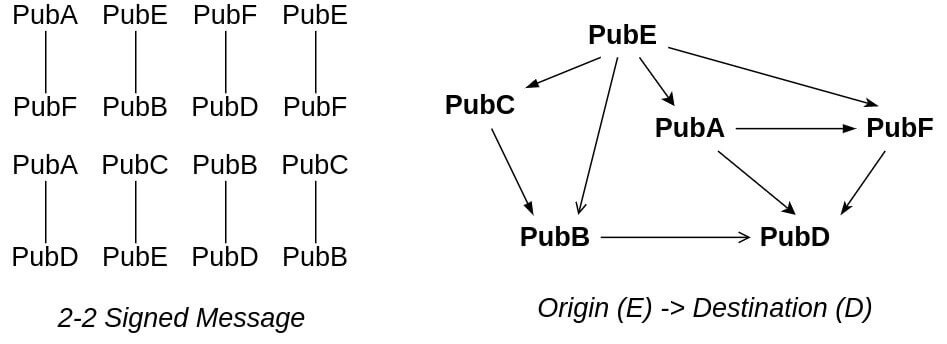
\includegraphics[width=8cm]{topology}
\caption{Topology}
\end{center}
\end{figure}
Delivery of unconfirmed transactions to nodes play important role in finality. Shared Mempools collude the network with duplicated data that results in a poor choice of transactions to include in a block. Miners take only transactions with higher fees. A direct-messaging system should be deployed with messaging instructions specific to each party as opposed to a gossip network. Paths are attached with unconfirmed transactions directly from the constructed network graph available to all nodes with public keys as pseudonymous identities protecting privacy. Two peered parties mutually sign a 2-2 random message for every $x$ block, and are gossiped across the network to identify the connection as online. From all the signed random messages proving each pubkey signature can display a network topology map from a node's point of reference. Paths are end to end encrypted with routing instructions that cannot trace back the origin. Nodes route transactions to the destinations where producers can attach the transaction to their allocated block. Since the stake information is available in the public ledger, client wallets can construct transactions along with path information that routes to nearest blocks for instant finality. Transactions are always atomic providing solution to queueing issues. Responsibilities are provided to all participants where nodes only receive the transactions which they need to include and client wallets should construct shorter paths to provide the best user experience.
\section{Propagation}
\begin{figure}[H]
\begin{center}
\includegraphics[width=11cm]{Snips}
\caption{Snips}
\end{center}
\end{figure}
A Block is collectively validated but constructed as snips - divisible block chunks by the producer and directly messaged to most of the current epoch's producer nodes with routing instructions to gossip across the network. Each snip references the previous snip's hash similar to the chain of blocks for proper identification of each block's snips. For a block of an epoch, a competition to deliver all snips under $x$ time intervals is required to win rewards and avoid slashing of fees. When a block fails to win it will not mint its last of snips which will contain the fees and rewards. VDF proofs are attached for every snip during routing to declare the state of each block's competition and resolve forks. Failed block fees and rewards are slashed by sending them to a burn address when blocks get confirmed by the producers. Each failed block with various categories shall result in decreased block production for the node in the next epoch by adding negative weights which indirectly slashes the bandwidth costing capital which instructs nodes to act honestly with the performance required for the epoch. Null-Blocks are self-minted by validators. Positive weights are given as an incentive for honest and notale performance during the epoch production. 

To synchronize time, each node's hash rate per second of a specific hash function is proved cryptographically onchain and taken in multiples of a common hardware's hash rate $(R)$ . This Individual hash-rate proof is also provided along with bandwidth proof for every epoch which trustlessly synchronizes all nodes as a single hardware producing continuous hashes concated with all snips. This provides cryptographic timestamped proofs to announce each epoch's block time under which all snips have to arrive and win the time-based propagation competition. The competition is termed "Proof of Speed".
\section{Rewards}

Rewards are given for each snip hash concated with transactions validated by VDF proofs. Since newly minted bitcoins for a period of time is definite and each epoch's sum of all block time is capped, new bitcoins can be supplied exactly proportional to the current Bitcoin issuance rate with halving. Each hash represents work done by nodes on validating and propagating transactions. When fork arises due to rejected snips, rest of block time and its allocated rewards are slashed. Meanwhile when a block is fully minted, rest of it's allocated rewards are distributed to next of block producers of the epoch. This encourages nodes to attest VDF proofs for receiving snips at earliest. While Tax outputs are attached as zero input transactions within the snip it contains, the rewards and fee outputs when accounted as a seperate snip marks the end of a block. 

During staking, producers announce their accepted tokens for which they will directly withdraw the commission. For other tokens, delegators can stake with a condition that their stake in bitcoins or the accepted stake token will be traded for the collected fees. During the commission withdrawal of non-accepted tokens, the producer will deposit collected fees to delegators and inflate the stake 1:1 ratio to withdraw the collateral. Users can pay in any token, delegators incur the risk, and producers get paid in tokens of their choice to validate transactions.
\section{Renting}
\begin{figure}[h]
\begin{center}
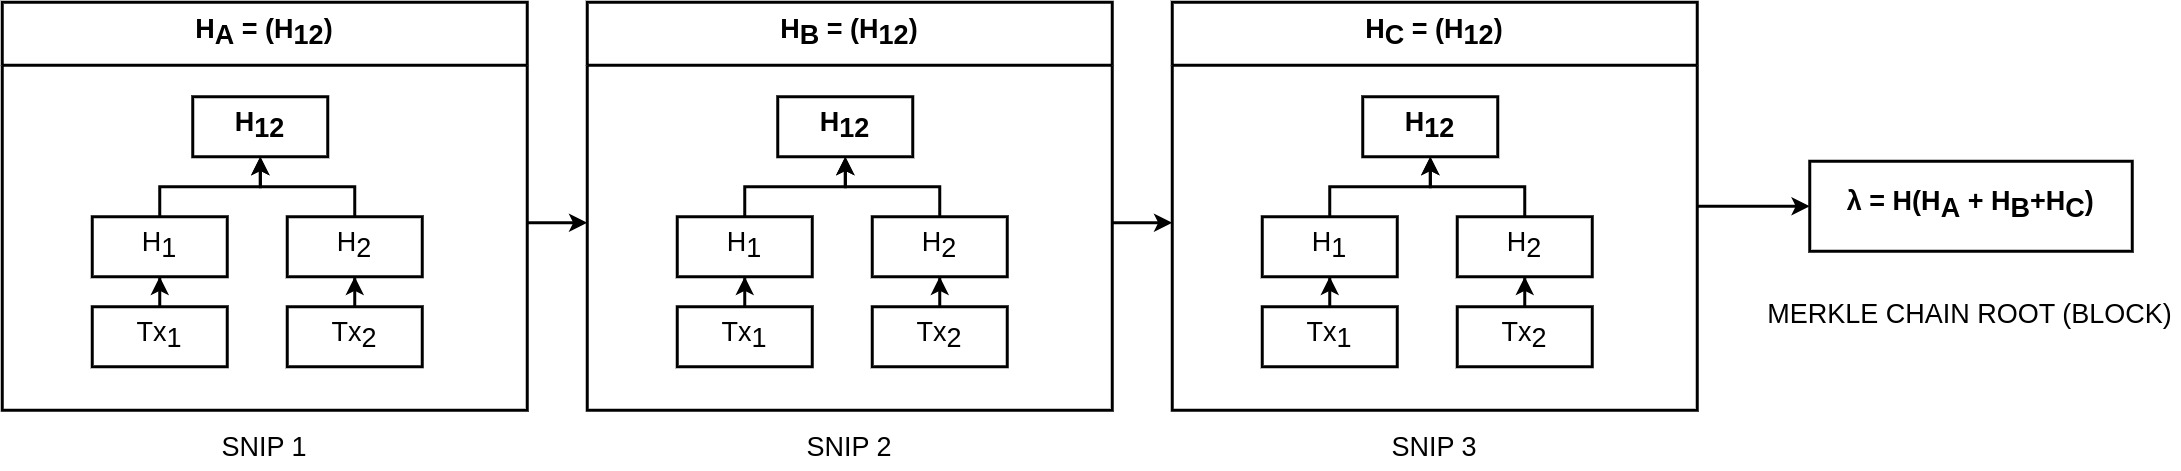
\includegraphics[width=13cm]{merklechain}
\caption{Merkle Chain}
\end{center}
\end{figure}
Instead of taking the Merkle roots of all the transactions inside a block, a snip's Merkle root is taken and linearly hashed to find the Merkle Chain root. Since snips can be rejected by validators, it is unsure to predict a Merkle chain root giving it a purely randomized value. Inside a snip contains parsed transactions whose hashes are taken to find the snip's Merkle root can be pruned if the UTXOs are spent, burnt, or expired. Each UTXO expiry block height is embedded in its script, and can be scanned by nodes, and pruned to optimize their data storage. Client Wallets can store each of their users' transaction history and can be audited onchain using Merkle chain roots. Renting rates can be given in market price independently voted by producer nodes for every epoch per byte per block. Users cannot directly pay for rent, but rather each new UTXO created is charged a transfer fee in the range of 0.05\% - 0.005\% decided based on the total volume of all transactions settled on previous epochs.
\begin{equation*}
5 \cdot 10^{-4} \leq \Delta f \leq 5 \cdot 10^{-5} == \sigma [\Psi (\epsilon_{n-3}, \epsilon_{n-2})] > 0.75
\end{equation*}
\begin{equation*}
f'=f+x \begin{cases}
x=+5 \cdot 10^{-6}, & \text{if } \Psi (\epsilon_{n-3} > \epsilon_{n-2})\\
x=-5 \cdot 10^{-6}, & \text{otherwise}
\end{cases}
\end{equation*}
\begin{conditions}
F & UTXO value $\times f'$ 
\end{conditions}
 Transfer fee charges more fees for higher value utxos and less for lesser value utxos bringing ease to transact for retailers. According to how much each utxo pays for a transfer fee, an expiry date is set. UTXOs doing state updates will not be charged and can combine UTXOs to a single balance holding UTXO with increased expiry value. This encourages users to store a single UTXO per wallet reducing transaction fees and also incentivizes nodes, clients, etc by saving disk space.  
\section{Forks}
\begin{figure}[H]
\begin{center}
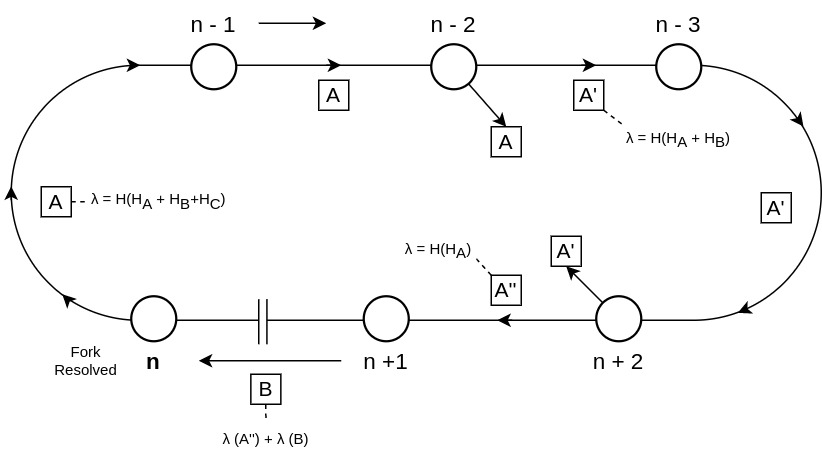
\includegraphics[width=10cm]{fork}
\caption{Resolving Forks}
\end{center}
\end{figure}
Confirmed blocks as snips are streamed with an included path that propagates across every producer in a backward ring manner. The snips are attached with VDF proofs by producers which provide proof of block time. Forks arise when different producers reject extra snips, this can be resolved by the very next block, providing instant finality to users. Additionally, negative weights are added if the fork arises after the first destination node of the path with VDF evaluation and also if a producers VDF proof isn't attested which directly denoes offline activity. In such cases producers construct new paths to deliver the snips. Block size and time is decided on consensus per epoch to prevent forks, which denotes a healthy propagation. Bandwidth upgrades are needed for the nodes which initiate the fork and directly instructs the origin block size should be decreased. 
\begin{align*}
\lambda (B_A) = H(H_A+H_B+H_C) \\
\lambda (B_{A'}) = H(H_A+H_B)\\
\lambda (B_{A''}) = H(H_A)  \\
\lambda (B_{B}) = H(\lambda(B_{A^?}) + \lambda(B_{B^?}))
\end{align*}
For a block, possible Merkle Chain Roots are constructed and forks are resolved. The next blocks will have the input hash value of the previous block's Merkle Chain Root. To avoid influence by the first destination node, path planning can be randomized but must include the next block producer ($n+1$) as the final destination.
\section{Oracles}

Oracle data provide real-time market rates to unlocking scripts every x interval of blocks defined. Various oracle protocols fall to freeloading and duplication issues on trustless oracle systems. A per-feed subscription based price-oracle protocol is introduced with partipants - exchanges, nodes, and users. Exchanges provide real-time market rates along with traded volume for weighted agregation of data. Nodes subscribe per request to exchange's price feeds for each token to increase positive weights as an incentive that assists in next of epoch election. Each exchange's feeds will have reputation scores that works similar to prediction markets maintained by users to avoid faulty data.

\section{Treasury}
For the active development and sustainability of the project, a DAO Treasury is set up to fund developers and the community. A minimal commission is imposed on producer fees and deposited to a treasury script. Memberships are non-fungible and non-transferable 1.Temporary (Core-Developers), 2.Permanent (Investors, Community), 3.Contracts (Employees, Operations). Each has its privileges provided to developers, investors, and community members. 

Votes can decide to add or remove contracts stating $x$ amount per $y$ term for $z$ period withdrawn during payouts. Votes can also decide to kick a temporary member due to any circumstantial issues or failure in active contribution. Permanent members cannot be kicked out due to their external contribution to building the project. Permanent and Temporary members cannot be added after genesis epoch but can appoint heirs to their membership. Contracts are paid out initially and the rest is provided to other memberships as dividends according to their weight. Core-Developers are only rewarded for their active-contribution, not indefinitely like holding a fungible token. A decentralized open-sourced organization structure is maintained with decisions involving votes brings forth a sustainable growth for the future of project blink. 
\section{Future}

The future of Bitcoin includes building L1 applications such as exchanges, bridges, lending \& borrowing, insurance, and mirrored wallets with current banking. Since these applications are developed inside an unlocking script, it requires preimage construction off-chain and settles onchain - inheriting the security of Bitcoin that centralized applications don't offer. Privacy can be improved by obscuring amounts and including ring signatures similar to Monero assisting regulators and masking financial information of a specific country. 

Since Layer 1 is dynamically scalable, the need for an offline-based off-chain digital cash-payment system will be developed with suitable hardware wallets. To provide a decentralized programmable environment, EVM will be deployed as a layer that can update its global-state \& contract state by providing a gas limit through a receipt-proof paid in any token. These EVM contracts shall not contain balances and EOAs, but rather purely for logic such as building DApps without a financial scope. Room for further improvement resides on sharding and size optimized scripts upgraded to Bitcoin and EVM Layer. Moreover reserach will be conducted to merge various bitcoin and altcoin chains for a clean experience on whole of finance and computing.\\

\noindent Implementations can be contributed openly to \url{https://github.com/projectblink}
\nocite{nakamoto2008bitcoin} \nocite{poon2016bitcoin}  \nocite{yakovenko2018solana} \nocite{wood2014ethereum}
\bibliographystyle{ieeetr}
\bibliography{citation.bib}

\noindent \textbf{Special Thanks}
\begin{itemize}
\item \textbf{Core-team} : \textit{Ajay Joshua, Shantanu Gaikwad, Aditya K Pandey, Sunidhi Sharma, Naveen Jose, Samarth Kulkarni}. 
\item \textbf{Advisors} : 
\end{itemize}

\newpage
\appendix
\noindent \Large \textbf{Appendix}
\normalsize
\section{Zk Circuits}
\subsection{Bandwidth Proof}
%Purva
\subsection{VoC Vote}
%Purva
\subsection{Hashrate Proof}
%Purva
\section{Election}

\subsection{Partcipation}

For every epoch before the allocation of blocks, the joining  requirement is increased by eliminating certain node's bandwidth proof by conducting a vote with current producers.

\begin{equation*}
|\mathbb{R}| = \{P(b)_1,P(b)_2,...P(b)_n\} 
\end{equation*}
Vote Participants,
\begin{equation*}
\forall |\mathbb{R}| \begin{cases}
|\mathbb{R}| \backslash \{\{P(b)_n\}\} \wedge \in |\mathbb{R}'|, & \text{if } P(b)_n < \bar{x}(|\mathbb{R}|) \\
P(b)_n \in |\mathbb{R}|,  & \text{otherwise}
\end{cases}
\end{equation*}
After Seed,
\begin{equation*}
\forall \mathbb{R'} k = \sum_{P(b)'_n \in |\mathbb{R}|} P(b)'_n
\end{equation*}
\begin{equation*}
\forall \mathbb{R'} \begin{cases}
|\mathbb{R}'| \backslash \{\{P(b)_n\}\}, & \text{ if } k > \bar{x}(|\mathbb{R}|) \cdot (51 \cdot 10^{-2})\\
P(b)_n \in |\mathbb{R}'|, & \text{ otherwise}
\end{cases}
\end{equation*}
Results, 
\begin{equation*}
|\mathbb{R}| = |\mathbb{R}| {\displaystyle \cup } |\mathbb{R}'|, i = \bar{x}(|\mathbb{R}|), |\mathbb{R}|=\emptyset
\end{equation*}
\begin{conditions}
|\mathbb{R}| & Block Producers\\
P(b)_n & PubKey's Bandwidth in bps \\
\bar{x} & Mean value\\
|\mathbb{R}''| & Producers to be voted\\
P(b)'_n & Voted Pubkey's bps\\
i & Joining requirement in bps 
\end{conditions}

\subsection{Producer Allocation}

Blocks are allocated for a whole epoch from a definite randomized seed where nodes constructs the same predictable result. Each producer's bandwidth proof $> i$ will provide the production rate in number of blocks.

\begin{equation*}
\text{Currently }|\mathbb{R}| = \emptyset, 
\text{If } \epsilon_{(n)}\{P(b)_n...\} > i \in |\mathbb{R}|
\end{equation*}
Block Size / sec,
\begin{equation*}
\epsilon_{n}(j)=min(|\mathbb{R}|) \cdot l
\end{equation*}
Weights addition,
\begin{equation*}
\forall |\mathbb{R}|, P(b)_n = \sum w(P) + P(b)_n = P(w)_n  \in |\mathbb{R}''|
\end{equation*}
Allocation,
\begin{equation*}
\forall |\mathbb{R}''|, \lfloor \Phi_{n} \rfloor = \frac{x \cdot P(w)_n}{10^4 \cdot \sum_{P(w)_n \in |\mathbb{R}''|} P(w)_n} \in |\mathbb{N}|
\end{equation*}

\begin{conditions}
x & Number of blocks per epoch\\
l & Latency\\
w & Individual weights\\
\Phi & Allocated number of blocks per producer\\
|\mathbb{R}''| & Producers with weight \\
|\mathbb{N}| & Producers with number of blocks allocation

\end{conditions}

\subsection{Random Seed}

To randomize the election, between a block range, a seed($k$) - Merkle Chain Root from a confirmed block is found. This seed should lie between a selected range in $2^{256}$ base10 possibilities. Difficulty rate is adjusted every epoch to seed entropy. If seed is not found, the last block of the range's MCR is taken. 

\begin{equation*}
|\mathbb{S}|= \{1,..2^{256}\} \text{ where, } k \in |\mathbb{S}|
\end{equation*}
\noindent Range Identify,
\begin{equation*}
|\mathbb{F}| = \{[(\frac{p}{d} \cdot q)+h],...(p=2^{256})\} \equiv |\mathbb{S}|
\end{equation*}
\begin{equation*}
h = 0, \text{ } h++ ;\text{ } q = 0, \text{ } q++ \text{ every } \frac{p}{d}
\end{equation*}
Value k,
\begin{equation*}
|\mathbb{X}| = \{[(\frac{p}{d} \cdot q)+h],...[(\frac{p}{d} \cdot q)+h]\}, 
\end{equation*}
\begin{equation*}
\text{ where } q \leq k' \leq q \in |\mathbb{X}|\subset |\mathbb{F}|
\end{equation*}
Difficulty level,
\begin{equation*}
k_{10} \text{ is taken} \begin{cases}
d = 1, k=k' ,     & \text{ if } k' \text{ is } ¿, \exists k \in |\mathbb{X}| \\
d++, k=k' ,       & \text{ if } \exists k \in |\mathbb{X}|\\
d-- \geq 2, k=k', & \text{if } \neg \exists k \in |\mathbb{X}| \vee \exists k \in |\mathbb{F}|\{p\}
\end{cases}
\end{equation*}
%\begin{equation*}
%where k is taken
%\end{equation*}
Block height allocation,
\begin{equation*}
Z_{16} = MD160_{16}((SHA256_{16}(k_{16}+b_h+\epsilon_h))
\end{equation*}
\begin{equation*}
Z_{16}
\begin{cases}
b_h++, P(\Phi_n) \in |\mathbb{L}|, \Phi_n = \Phi_n-1 \in |\mathbb{N}|,   &  \text{ if } |\mathbb{N}| \neq \emptyset \wedge \forall \Phi_n \in |\mathbb{N}| < Z_{16} \\
MD160_{16}(Z_{16}),  & \text{ if } |\mathbb{N}| \neq \emptyset \wedge \forall \Phi_n \in |\mathbb{N}| > Z_{16} \\
|\mathbb{N}| \{\Phi_n\} \backslash  |\mathbb{N}|, & \text{ if } \Phi_n=0\\
\{n(|\mathbb{L}|)+1,..x\}=|\mathbb{L}|\Phi_n =\{1,..\},  & \text{ if } |\mathbb{N}| = \emptyset  \wedge x-n(|\mathbb{L}|)=\mathbb{N}\\
|\mathbb{L}|,   & \text{ if } |\mathbb{N}| = \emptyset \wedge n(|\mathbb{L}|)=x
\end{cases}
\end{equation*}
Block Time,
\begin{equation*}
\epsilon_n b(\tau) = \widetilde{x}(\epsilon_{n-2}(b_1^x)) \in |\mathbb{B}|
\end{equation*}
Block Size,
\begin{equation*}
Block size here (b_s)
\end{equation*}
\begin{conditions}
b_h & Block height in base$_{10}$\\
\epsilon_h & Epoch height in base$_{10}$\\
P(\Phi_n) & Pubkey in MD160 base$_{16}$ rep
\end{conditions}
\section{Taxes}
During the unlocking script stack execution, with the solutions offered by sCrypt to take the preimage of the entire transaction, the outputs are validated with aaccuracy of providing the capital gains tax to the regulating authority of the unlocking script. Capital gains are imposed to the profits by feeding from an onchain oracle for the token id. Profits are calculated from the time of minting the script to spending. TDS or Tax Deducted at Source, a fixed percentage of a entire balance can be imposed by employers and payers to payees. It restricts the TDS amount when the script balance is spent and sends to the regulator. Sales tax is direct tax payment with two outputs imposed when a product is bought where the merchant provides information about the tax amount with its regulator and the price excluding the tax paid to merchant. Implementations can be contributed to \url{https://github.com/projectblink/Blink_sCrypts} 
\section{Stake Proof}
\subsection{Deposit}
Delegators can provide their bitcoins or the accepted token for staking to node's publicly available stake script for a specific accepted token id. For Non-accepted tokens stake script can be created by delegators themseleves and add the nodes information to it. 
%\begin{equation*}
%stake to script of tokenid, accepted staking token id and node pubkey which will have a limit, or create a script for node pubkey with tokenid, accepted staking token id. Node pubkey cannot withdraw, rather it can freeze during his own block. Users can freely deposit with pubkey and withdraw to same pubkey or withdraw to any pubkey.
%\end{equation*}
This stake script will have public functions such as deposit, withdraw, freeze called by delegators and the node. Stakes can be freezed by authorized node restricting deposit and withdrawal for the block it is collateralized. 
\subsection{Fee}
Fees are provided to Delegators, Validators and DAO Tresury. The rules for withdrawing are different for accepted and non-accepted tokens as validators should have their independent choice of payout tokens to provide service to users.
%\begin{equation*}
%Direct withdrawal of commission, and dao payout and then depositing fees to stake script. 
%\end{equation*}
%\begin{equation*}
%Depositing fees, inflating ratio and making node as a delegator and dao script as a delegator too.
%\end{equation*}
\subsection{Withdrawal}
All delegators can able to withdraw the available tokens according to their weight of stake.
%\begin{equation*}
%Withdrawal ratio
%\end{equation*}

\section{Routing Path}
%Path with nlocktime, encryption, onion mixing, secret number, path layers
%Purva

\section{Hash-Reward}
Halving of Bitcoin issuance is done every $R \cdot (1.26 \cdot 10^8)$ hashes equals 210,000 of 10-minute bitcoin blocks. Every epoch ($\epsilon_n$) will have a $g$ amount of bitcoins to be issued. Hence for every epoch a target $g(\epsilon_n)$ new bitcoins is set to mint. For forked blocks, the supply is slashed. For fully minted blocks with remaining hashes, the rewards are distributed to next hashes equally incentivizing producers.
\begin{equation*}
g[R(\epsilon_n)] = \frac{\Delta g(\epsilon_n)}{\epsilon_n(\sum_1^n R)}
\end{equation*}
Rewards per block,
\begin{equation*}
g[R(\epsilon_n(b))] = \epsilon_n(b(\sum_1^n R)) \cdot g[R(\epsilon_n)]
\end{equation*}
\begin{equation*}
\Delta g(\epsilon_n) = g(\epsilon_n) - [\sum_1^n g[R(\epsilon_n)]  \in b(\epsilon_n)]
\end{equation*}
Finding forks $\Delta \lambda$,
\begin{equation*}
\forall \epsilon_n(b_n), \Delta g(\epsilon_n) = 
\begin{cases}
g(\epsilon_n) - g(\epsilon_n(b_n)), & \text{ if } \Omega(b_n) =  0 \\
\Delta g(\epsilon_n) + b, & \text{ if } \Omega(b_n) = \mathbb{N} \wedge \lambda  \\
\Delta g(\epsilon_n) - b, & \text{ if } \Omega(b_n) =  \mathbb{N} \wedge \Delta \lambda \\
\end{cases}
\end{equation*}
\begin{equation*}
\Omega(b_n) = g(\epsilon_n(b)) - [\sum_1^n g[R(\epsilon_n)]  \in b_n(\epsilon_n)]
\end{equation*}
\section{VDF Proof}
%Joby
\section{Weights}
Weights are provided to slash oppurtunity for producing blocks in next epochs for dishonest, lower performance node which fails to mint the block fully, or create forks due to lower bandwidth. Each weight shall increment or decrement the posted bandwidth costing capital to nodes.
\begin{align*}
\text{Null Block} = -0.015 \cdot (\widetilde{x}|\mathbb{R}|)\\
\text{Fork$^{1deg}$} = -0.005 \cdot (\widetilde{x}|\mathbb{R}|)\\
\text{Forks$^{2deg}$} = -0.07 \cdot (\widetilde{x}|\mathbb{R}|)\\
\text{Fork Proof$^{1deg}$} = +0.005 \cdot (\widetilde{x}|\mathbb{R}|)\\
\text{Fork Proof$^{2deg}$} = +0.07 \cdot (\widetilde{x}|\mathbb{R}|)\\
\text{Age} = +0.03 \cdot (\widetilde{x}|\mathbb{R}|)\\
Extras here
\end{align*}
Null Block weight is added if a producer fails to add a block with no snips. Forks of degree 1 refers to the fork created by the first destitation producer after receiving the snip, imposed on the block producer. Forks of degree 2 refers to the fork created by further destinations. Both the sender and receiver shall incur the negative weight equally shared during forks. Fork proofs can be provided by anynode usually the producer before the fork, who are incentivized for their honesty. Age is a positive weight provided to producers who mint blocks without forks for entire the epoch.
\section{Oracle}
%Joby
\section{DAO}
%Joby
% To remove a temporary member - Vote percentage - (Temporary members 100\% (except the member to be removed ), Permanent Members 0\%, Employees - 75\%) - Period is first 20 days of the month
%To remove a contract -(Temporary members - 51\%, Permanent members - 0\% (can vote), Employees - 51\%) - Period is last 10 days of the month
% To include a contract (Temporary members - 51\%, Permanent members - 0\% (can vote), Employees - 51\%) - Period is first 20 days of the month
\section{Size Optimization}
\section{Improvements}
%emphasis on zkpart of election and verifying the snips produced by the node without knowing their full identity until the full block is minted.
\end{document}